
% This LaTeX was auto-generated from MATLAB code.
% To make changes, update the MATLAB code and republish this document.

\documentclass{article}
\usepackage{graphicx}
\usepackage{color}

\sloppy
\definecolor{lightgray}{gray}{0.5}
\setlength{\parindent}{0pt}

\begin{document}

    
    \begin{verbatim}
clear;clc

A = [0 1 0 0; 0 0 1 0; 0 0 0 1; -650 -180 -90 -6];
B = [0; 0; 0; 1];
C = [90 15 10 0];

eig(A)

cm = ctrb(A,B);
rank(cm)
om = obsv(A,C);
rank(om)

x(:,1) = [2; 1; 3; 0];
y(:,1) = C*x(:,1);
x_cl(:,1) = [2; 1; 3; 0];
y_cl(:,1) = C*x_cl(:,1);
x_hat(:,1) = [0; 0; 0; 0];
y_hat(:,1) = C*x_hat(:,1);

t = 0:0.01:10;
nt = length(t);
dt = t(2) - t(1);
% input
for i = 1:nt
    r(:,i) = 1;
end

Ts = 2;
Mos = 2;
Mlog2 = log(Mos/100)^2;
zeta = sqrt(Mlog2/(Mlog2 + pi^2));
omegaN = 4/(Ts*zeta);

p1 = -zeta*omegaN + 1i*omegaN*sqrt(1-zeta^2);
p2 = -zeta*omegaN - 1i*omegaN*sqrt(1-zeta^2);

P = [p1;p2;-2;-7]
K = place(A,B,P); % K = [ -557.8852  -64.7834  -33.4204    7.0000];
eig(A-B*K)
P1 = [-0.5+1i;-0.5-1i;-2;-100]
L = place(A',C',P1); L = L'
eig(A - L*C)

for i = 1:nt-1
x_dot(:,i) = A*x(:,i)+B*r(:,i);
x(:,i+1) = x(:,i) + x_dot(:,i)*dt;
y(:,i+1) = C*x(:,i+1);
x_cl_dot(:,i) = (A-B*K)*x_cl(:,i) + B*r(:,i);
x_cl(:,i+1) = x_cl(:,i) + x_cl_dot(:,i)*dt;
y_cl(:,i+1) = C*x_cl(:,i+1);
x_hat_dot(:,i) = (A-B*K)*x_hat(:,i)+L*(y_cl(:,i)-C*x_hat(:,i)) + B*r(:,i);
x_hat(:,i+1) = x_hat(:,i) + x_hat_dot(:,i)*dt;
y_hat(:,i+1) = C*x_hat(:,i+1);

end
figure
plot(t,r,'k--',t,y,'r-.',t,y_cl,'b-',t,y_hat,'m-','linewidth',2)
set(gca,'fontsize',18)
legend({'step-input','y open-loop','y state-feedback','y observer integral'},'Interpreter', 'latex')
legend boxoff
xlabel('Time (s)')
\end{verbatim}

        \color{lightgray} \begin{verbatim}
ans =

  -2.0147 + 8.3137i
  -2.0147 - 8.3137i
  -0.9853 + 2.8128i
  -0.9853 - 2.8128i


ans =

     4


ans =

     4


P =

  -2.0000 + 1.6061i
  -2.0000 - 1.6061i
  -2.0000 + 0.0000i
  -7.0000 + 0.0000i


ans =

  -7.0000 + 0.0000i
  -2.0000 + 1.6061i
  -2.0000 - 1.6061i
  -2.0000 + 0.0000i


P1 =

   1.0e+02 *

  -0.0050 + 0.0100i
  -0.0050 - 0.0100i
  -0.0200 + 0.0000i
  -1.0000 + 0.0000i


L =

   -0.5290
    2.5976
   10.5645
  -76.1004


ans =

   1.0e+02 *

  -1.0000 + 0.0000i
  -0.0050 + 0.0100i
  -0.0050 - 0.0100i
  -0.0200 + 0.0000i

\end{verbatim} \color{black}
    
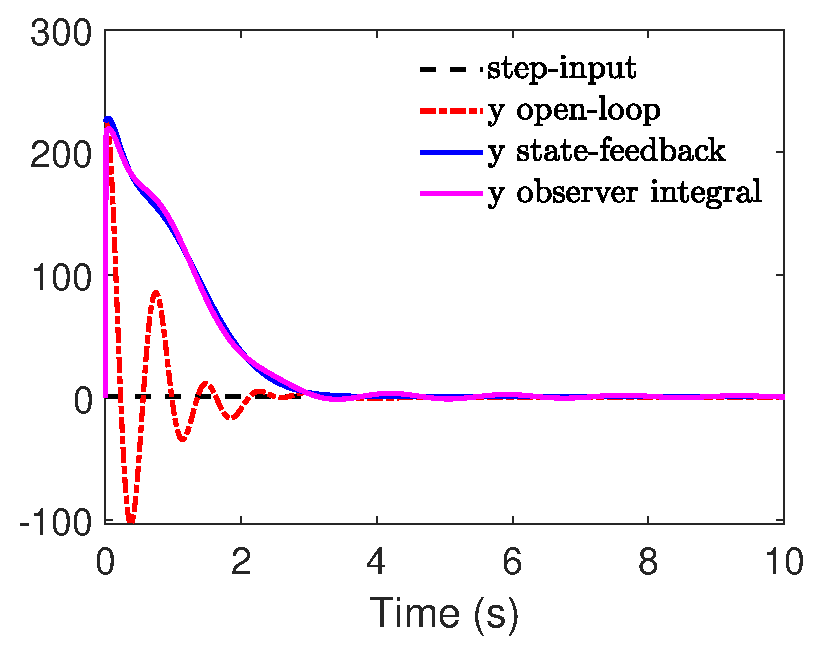
\includegraphics [width=4in]{hw8_2_2_01.eps}



\end{document}

